\section{Architecture}\label{arch}
\noindent This section presents the \sys architecture.

\subsection{Overview}\label{sysover}
Figure \ref{sys-arch} illustrates the \sys architecture.
The dotted boxes describe optional components that the user can provide to improve the efficiency of the system.  

\subsubsection{Required User Input}\label{uinp}
%To use \sys, the user provides the following:

\noindent\textbf{Model:} The user provides a predictive model (e.g., SVM) specified as a convex loss optimization problem $\phi(\cdot)$ and a featurizer $F(\cdot)$ that maps a record to its feature vector $x$ and label $y$.

\vspace{0.25em}

\noindent\textbf{Cleaning Function: } The user provides a function $C(\cdot)$ (implemented via software or crowdsourcing) that maps dirty records to clean records as per our definition in Section \ref{dmodel}. 

\vspace{0.25em}

\noindent\textbf{Batches: } Data are cleaned in batches of size $b$ and the user can change these settings if she desires more or less frequent model updates.
The choice of $b$ does affect the convergence rate.
Section~\ref{model-update} discusses the efficiency and convergence trade-offs of different values of $b$.
We empirically find that a batch size of $50$ performs well across different datasets and use that as a default.
A cleaning budget $k$ can be used as a stopping criterion once $C(\dot)$ has been called $k$ times, and so the number of iterations of \sys is $T = \frac{k}{b}$.
Alternatively, the user can clean data until the model is of sufficient accuracy to make a decision.

\subsubsection{Basic Data Flow} \label{df}
The system first trains the model $\phi(\cdot)$ on the dirty dataset to find an initial model $\theta^{(d)}$ that the system will subsequently improve.
The {\it sampler} selects a sample of size $b$ records from the dataset and passes
the sample to the {\it cleaner}, which executes $C(\cdot)$ for each sample record and outputs their cleaned versions.
The \emph{updater} uses the cleaned sample to update the weights of the model, thus moving the model closer to the true cleaned model (in expectation).
Finally, the system either terminates due to a stopping condition (e.g., $C(\cdot)$ has been called a maximum number of times $k$, or training error convergence),
or passes control to the {\it sampler} for the next iteration.

\subsubsection{Optimizations}
In many cases, such as missing values, errors can be efficiently detected.
A user provided {\it Detector} can be used to identify such records that are more likely to be dirty, and thus improves the likelihood that the next sample will contain true dirty records.
Furthermore, the {\it Estimator} uses previously cleaned data to estimate the effect that cleaning a given record will have on the model.
These components can be used separately (if only one is supplied) or together to focus the system's cleaning efforts on records that will most improve the model.
Section \ref{opti} describes several instantiations of these components for different data cleaning problems.
Our experiments show that these optimizations can improve model accuracy by up-to 2.5x (Section \ref{comp}).

\subsection{Example}
The following example illustrates how a user would apply \sys to address the use case in Section~\ref{s:usecase}:
\begin{example}\label{archex}
The analyst chooses to use an SVM model, and manually cleans records by hand (the $C(\cdot)$).  
\sys initially selects a sample of $50$ records (the default)  to show the analyst.
She identifies a subset of 15 records that are dirty, fixes them by normalizing the drug and corporation names with the help of a search engine, and corrects the labels with typographical or incorrect values.
The system then uses the cleaned records to update the the current best model and select the next sample of $50$.
The analyst can stop at any time and use the improved model to predict donation likelihoods.
\end{example}






\iffalse
  \noindent To summarize in pseudocode:
  \begin{enumerate}[leftmargin=1em]\scriptsize\sloppy
  \item \texttt{Init(dirty\_data, cleaned\_data, dirty\_model, batch, iter)}
  \item For each t in $\{1,...,T\}$
  \begin{enumerate}
    \item \texttt{dirty\_sample $=$ sampler(dirty\_data, sample\_prob, detector, batch)}
    \item \texttt{clean\_sample $=$ Cleaner(dirty\_sample)}
    \item \texttt{current\_model $=$ Update(current\_model, sample\_prob, clean\_sample)}
    \item \texttt{cleaned\_data = cleaned\_data + clean\_sample}
    \item \texttt{dirty\_data = dirty\_data - clean\_sample}
    \item \texttt{sample\_prob $=$ Estimator(dirty\_data, cleaned\_data, detector)}
    \item \texttt{detector $=$ DetectorUpdater(detector, cleaned\_data)}
  \end{enumerate}
  \item \texttt{Output: current\_model}
  \end{enumerate}
\fi


\iffalse
  \subsection{Challenges and Formalization}
  We highlight the important components and formalize the research questions explored in this paper. 

  \vspace{0.5em}

  \noindent\textbf{Detector (Section \ref{det}). } The first challenge in \sys is dirty data detection. In this step, the detector selects a candidate set of dirty records $R_{dirty} \subseteq R$. There are two techniques to do this: (1) an \emph{a priori} case, and (2) and an adaptive case. In the \emph{a priori} case, the detector knows which data is dirty in advance. In the adaptive case, the detector learns classifier based on previously cleaned data to detect corruption in uncleaned data.

  \vspace{0.5em}



  \vspace{0.5em}



  \vspace{0.5em}

  \noindent\textbf{Update (Section \ref{model-update}). } This step updates the model $\theta^{(t)}$ based on the featurized (with featurization $F(\cdot)$) cleaned sample $F(S_{clean})$ resulting in $\theta^{(t+1)}$. Analyzing the model update procedure as a stochastic gradient descent algorithm will help derive the sampling distribution and estimation.

  \vspace{0.5em}

  \noindent\textbf{Estimator (Section \ref{sampling}): } The estimator approximates the optimal distribution derived in the Sample step. Based on the change in the featurized data $F(S_{clean})$ and $F(S_{dirty})$, it directs the next iteration of sampling to select points that will have changes most valuable to the next model update.


  \subsection{Optimizations}
  There are three aspects of \sys, that allow us to achieve this design point: error partitioning, gradient-based model update (Section \ref{model-update}), estimate-driven sampling (Section \ref{sampling}).

  \vspace{0.5em}

  \noindent\textbf{Partitioning Dirty and Clean Data: } In many applications, enumerating the set of corrupted records is much easier than cleaning them. For example, we may be able to select the set of rows that have missing values but actually filling those missing values is expensive. Likewise, in the constraint literature, selecting a set of rows that have a violated constraint can be done in polynomial time, however, fixing the constraints is NP-Hard.
  In our error detection step, we partition the dirty and clean data.
  Partitioning serves two purposes: (1) it reduces the variance of our updates because we can cheaply scan over data we know that is clean, and (2) it increases the fraction of actually dirty records in the candidate batch.
  A good example of why we need the second objective is seen in the context of crowdsourcing.
  If we have a crowdworker clean records, we will have to pay them for the task whether or not the record required cleaning.
  To efficiently use this partitioning, we need a database solution indexing dirty and clean data.

  \vspace{0.5em}

  \noindent\textbf{Gradient-Based Updates: } In \sys, we start with a dirty model and then make an update using a gradient step. Here, we can draw an analogy to Materialized View maintenance, since after all, a model parametrized by $\theta$ is just a table of floating point numbers.
  Krishnan et al. proposed a technique called sample view cleaning, in which they take a clean sample of data and propagate the updates to a Materialized View.
  Similarly, in this work, we take the information from a sample of cleaned data and propagate an update with the gradient.

  \vspace{0.5em}

  \noindent\textbf{Estimate-Driven Sampling: } Repair is the most expensive step in the workflow, so optimizing for scan cost may lead to negligible overall time improvements.
  We can sacrifice a small overhead in pre-computation for each data point to determine its value to the model and select a sampling distribution accordingly.
  Intuitively, while each iteration has an increased cost, it also makes more progress towards the optimum.


  \begin{example}

  The analyst first trains an SVM model on the dirty data ignoring the effects of the errors resulting in a model $\theta^{(d)}$.
  She decides that she has a budget of cleaning $100$ records, and decides to clean the 100 records in batches of 10 (set based on how fast she can clean the data, and how often she wants to see an updated result).
  She initializes \sys with $\theta^{(d)}$.
  \sys samples an initial batch of 10 records.
  She manually cleans those records by merging similar drug names, making corporation names consistent, and fixing incorrect labels.
  After each batch, the model is updated with the most recent cleaning results $\theta^{(t)}$.
  The model improves after each iteration.
  After $t=10$ of cleaning, the analyst has an accurate model trained with 100 cleaned records but still utilizes the entire dirty data.
  \end{example}
\fi

\begin{figure}[t]
\centering
 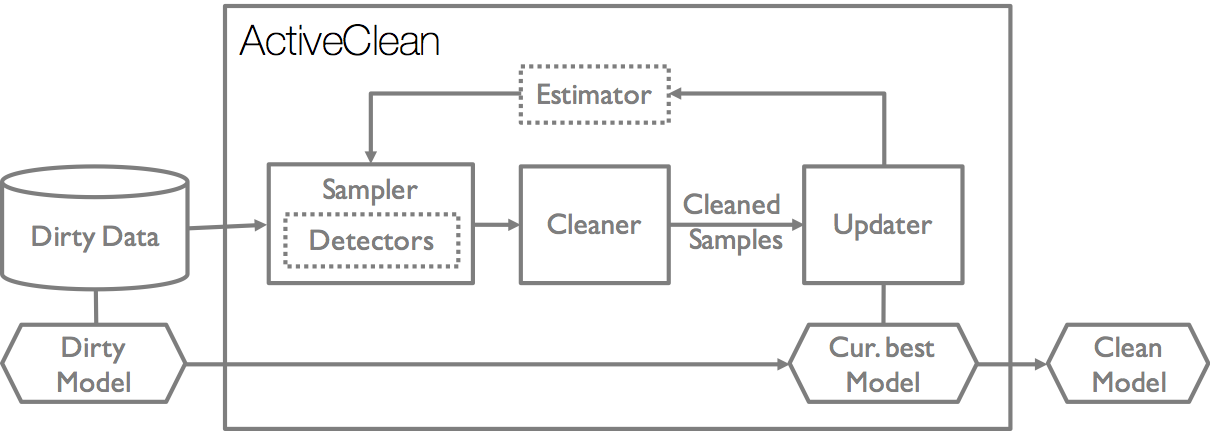
\includegraphics[width=\columnwidth]{figs/arch.png}
 \caption{\sysfull allows users to train predictive models while progressively cleaning data. The framework adaptively selects the best data to clean and can optionally (denoted with dotted lines) integrate with pre-defined detection rules and estimation algorithms for improved conference. \label{sys-arch}}
\end{figure}


